\section{Modeling \pp collisions}
Theoretical predictions of \pp collisions are an important tool for understanding physical processes and modeling observables studied at the LHC. These predictions are based on an underlying proton model and calculations are performed from approximations at different energy scales. Precision measurements such as the one in this thesis provide important information to further refine these models and calculations. This chapter describes the general methods for modeling proton-proton collisions as well as details about \W and \Z boson production at the LHC.
\subsection{Simulating \pp interactions}
In collisions at very low energies, protons can be approximated as electrically charged objects. At higher energies, such as those at the LHC, the structure within protons begins to have an important role for the scattering process. \W and \Z bosons are produced from the interaction of quarks and gluons (both also referred to as partons) within the proton\cite{PhysRevLett.23.930,PhysRevLett.23.935}. The contributions of the partons to the proton's structure are described by parton distribution functions (PDFs). The PDFs, $f_i(x,Q^2)$, give the probability of finding a parton of carrying a fraction $x$ of the proton's longitudinal momentum. Current PDFs are determined by global fits to experimental data sets\cite{Perez_2013} (recent advances in lattice QCD may ). Valence quarks, sea quarks, and gluons within the proton are described by the PDFs. 

For hard scattering processes such as \W and \Z boson production, the momentum transfer, $Q$ is high. Due to the asymptotic freedom of QCD, the coupling constant $\alpha_S(Q^2)$ is small, and perturbative calculations are effective. The highest order calculation currently available for the \W and \Z production is next-to-next-to-leading order (NNLO)\cite{Anastasiou:2003ds}. 

In the perturbative expansions, initial-state radiation of soft and collinear gluons produces logarithmic terms which cause singularities and divergences in the calculations. To accommodate this effect, the calculation can be split into perturbative and non-perturbative regimes. This is described by the factorization theorem, which ensures that the hard process is independent of the intial-state radiation, and separates the QCD calculations at a factorization scale, $\mu_F$. This allows the singularities due to the soft gluon emissions to be factored out and contained within the PDFs~\cite{Collins:1989gx}. The PDF dependence on the factorization scale is determined by the Dokshitzer–Gribov– Lipatov–Altarelli–Parisi (DGLAP) equations. The DGLAP equations introduce a $\mu_F$ dependence to the scale-independent PDFs by including initial-state soft radiation, and provide an evolution of the PDFs over different factorization scales\cite{Gribov:1972ri,Dokshitzer:1977sg}.  Equation~\ref{eq:factorization_xsec} shows the factorized cross section calculation. The first section includes the PDFs, $f_{a}$ and $f_{b}$, evaluated at the factorization scale $\mu_F$, for partons $a$ and $b$, each carrying fractions $x_a$ and $x_b$ of the proton momentum. The second half describes the hard scattering between the two partons, where the cross section, $\hat{\sigma}$, is expanded perturbatively.  
\begin{equation}
\begin{aligned}
\sigma_{p_a p_b \rightarrow n} &= \sum_{a,b}{\int{dx_a dx_b f_{a}(x_a, \mu^2_F)f_{b}(x_b, \mu^2_F)}} \\ &\times[\hat{\sigma}_{LO}(x_a x_b s, \mu^2_R, \mu^2_F)+\alpha_S \hat{\sigma}_{NLO}(x_a x_b s, \mu^2_R, \mu^2_F) + \cdots]
    \label{eq:factorization_xsec}
\end{aligned}
\end{equation}
% Parton-parton cross sections ($\hat{\sigma}$) are determined by numerically integrating matrix element calculations by using a Monte Carlo (MC) process to sample the phase space.

Matrix element calculation breaks down for soft and collinear final states. Instead, parton shower models are used to produce the final-states at non-perturbative scales. Showering is modeled as series of radiative steps, with partons branching into consecutively lower energy state: $q\rightarrow gq$, $g\rightarrow gg$, and $g\rightarrow q\bar{q}$ for QCD. Branching probability at a scale $Q^2$ is determined by evolving the splitting functions using the DGLAP equations. Additionally, QED interactions ($q\rightarrow q\gamma$ and $l\rightarrow l\gamma$) are included in the shower modeling. Parton showering continues to the scale $\Lambda\sim 200~\mathrm{MeV}$, where bare partons are hadronized into color-neutral hadrons. Then the unstable hadrons are decayed according to branching ratios. Factorization and a hard scatter process, along with subsequent parton showering and hadronization is illustrated in Figure~\ref{fig:sm:evtgen}.

% Multiple collaborations exist to provide tools capable of performing the different calculations described above. 

\begin{figure}
\centering
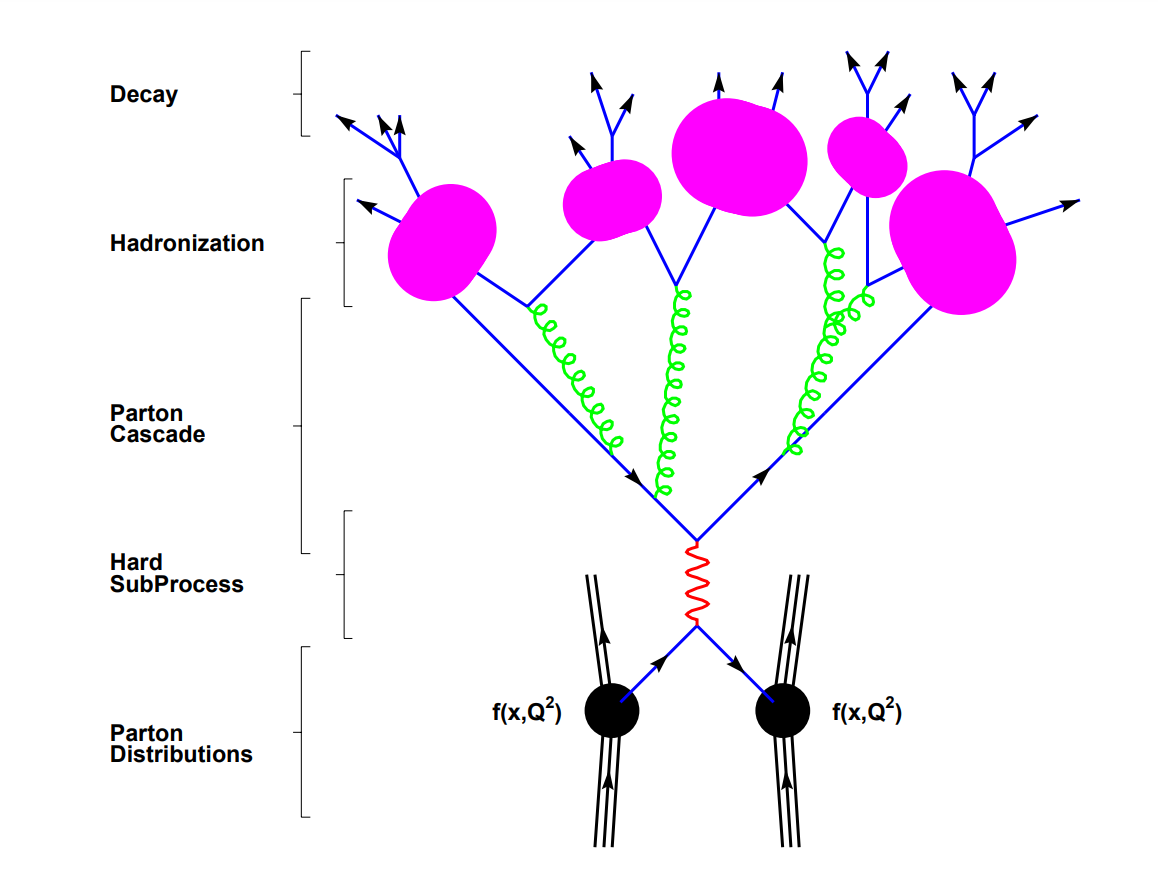
\includegraphics[width=0.6\linewidth]{plots/SM/evtgenerator.PNG}
%   \caption{1a}
%   \label{fig:Eff:el:5TeV:GSFSel:pos
\caption{Illustration of a hard-scatter process. \protect\cite{Dobbs:2001ck}}
\label{fig:sm:evtgen}
\end{figure}
% %%%%%%%%%%%%%%%% vvvvvvv finish later
% % %% Comment back in later 
\subsection{\W and \Z production at the LHC}
In the \pp collisions, the bosons are produced through the interaction of quarks and gluons within the protons. The primary production modes for the \W and \Z bosons is through the Drell-Yann process, predominantly $u\bar{u}, d\bar{d}\rightarrow Z$,  $u\bar{d}\rightarrow W^+$,  and $d\bar{u}\rightarrow W^-$. In proton-proton collisions, these processes require the participation of at least one sea quark \cite{PhysRevLett.25.316}. 

The kinematic variables describing the partons participating in the interaction are listed in Equations~\ref{eq:scattering_vars}. The mass of the boson is represented by $M$, the rapidity of the boson is represented by $y$, and \s is the center-of-mass energy of the collision. The relative fraction of the proton's longitudinal momentum held by each of the initial partons is represented by $x_1$ and $x_2$. 
\begin{equation}
\begin{aligned}
M &= \sqrt{x_1 x_2 s} \\ 
y &= \frac{1}{2} \ln \bigg( \frac{E+p_z}{E-p_z}\bigg) = \frac{1}{2} \ln \bigg( \frac{x_1}{x_2}\bigg)\\ 
x_1 &= \frac{M}{\sqrt{s}} e^{y},~ x_2 = \frac{M}{\sqrt{s}} e^{-y}
\end{aligned}
\label{eq:scattering_vars}
\end{equation}
% % %%%% figure
\begin{figure}
\centering
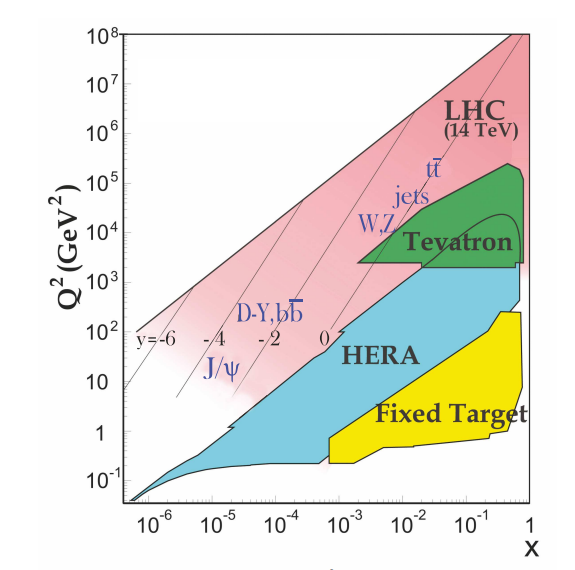
\includegraphics[width=0.6\linewidth]{plots/SM/structure_probes.PNG}
%   \caption{1a}
%   \label{fig:Eff:el:5TeV:GSFSel:pos
\caption{Phase space of Bjorken-x and $Q^2$ available at the LHC and other experiments. \pp collisions at the LHC can probe very high $Q^2$. \protect\cite{PhysRevD.98.030001}}
\label{fig:sm:summary:xVsQ2}
\end{figure}

\W and \Z boson production occupies a phase space near $Q \sim 100 \GeV$ (approximately the \W or \Z boson mass). Given a measurement acceptance of $|y| < 2.4$, this allows us to study $x$ approximately within the range $10^{-4} < x < 0.1$ at the LHC.

When simulating the proton-proton interactions, the PDFs describing the relative fraction $x$ of the proton's momentum contained by the individual partons is important. As previously described, the PDFs are dependent on the energy scale of the interaction, and in the case of the \W and \Z boson production this scale is around the mass of the bosons $Q\sim 100 \GeV$. There are many collaborations dedicated to providing PDF sets for use in these predictions, with many of the PDFs constructed from global fits to experimental data. Each collaboration uses a different approach and often different sets of experimental data in the fits, resulting in different PDF predictions and uncertainties. Inclusive \W and \Z production cross section measurements play and important role in PDF determination as they  An example illustrating the PDFs involved in \W and \Z boson production is given in Figure~\ref{fig:sm:nnpdf}\cite{Ball:2017nwa,Gao:2017yyd,Accardi:2016ndt,Butterworth:2015oua,Rojo:2015acz}.. 
\begin{figure}[htbp]
\centering
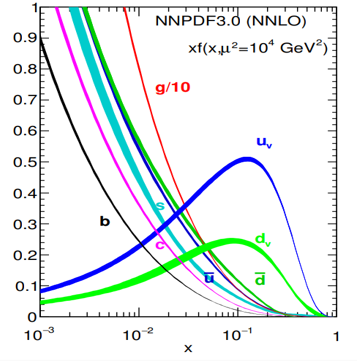
\includegraphics[width=0.6\linewidth]{plots/SM/PDFSET.PNG}
\caption{An example of a PDF illustrating the relative contribution of partons to the proton's longitudinal momentum at $Q\sim 100\GeV$, provided by the NNPDF collaboration\cite{Ball:2017nwa}. The valence quarks $u$ and $d$ are shown in bright blue and green, while the other quark flavors are sea quarks.}
\label{fig:sm:nnpdf}
\end{figure}.
An illustration of the involvement of the various quark flavors in the production of \W and \Z bosons at a range of rapidities is shown in Figure~\ref{fig:wz_rapidity}.  Measurement of \W production in proton-proton collisions allows for separation of quark flavors, and ratios of \W and \Z cross sections can provide constraint to the strange content of the proton. \begin{figure}[htbp]
\centering
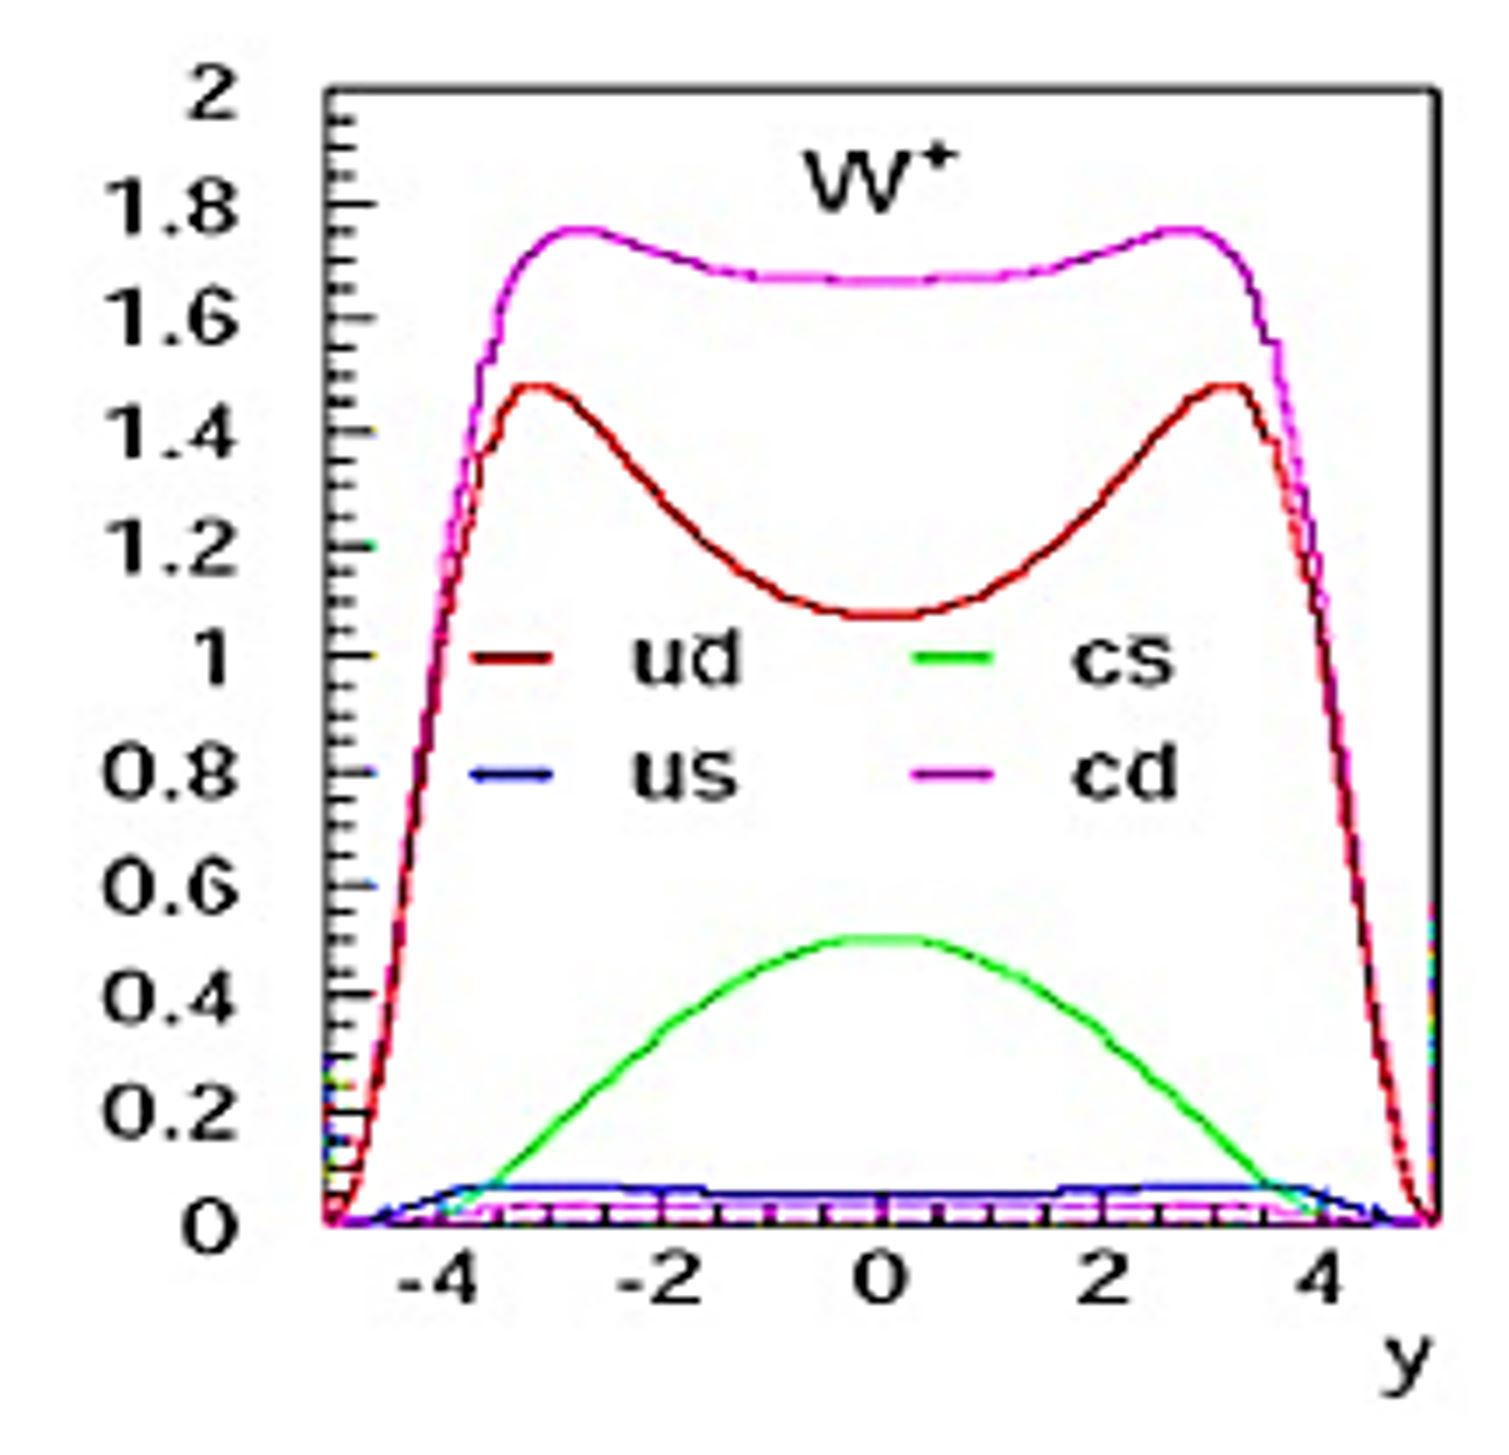
\includegraphics[width=0.31\textwidth]{plots/SM/rapidity_Wp.JPG}
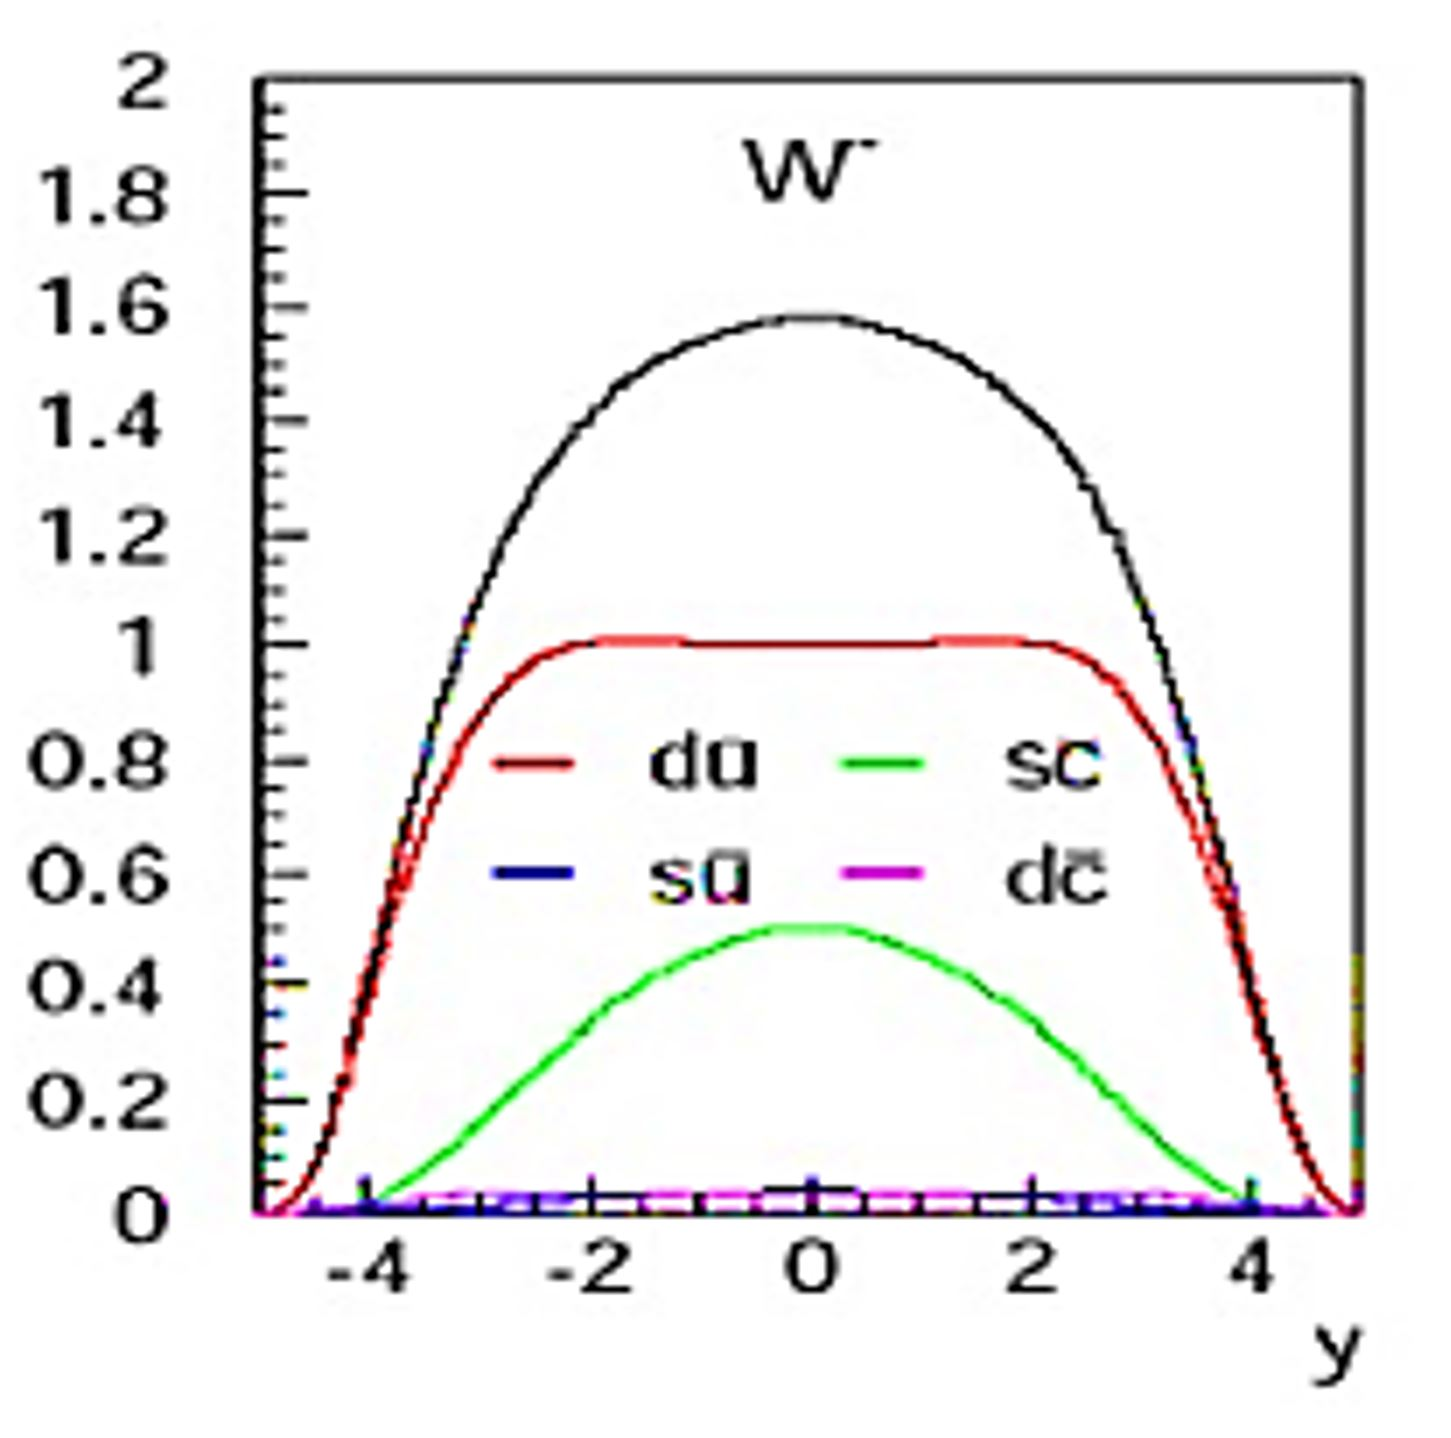
\includegraphics[width=0.30\textwidth]{plots/SM/rapidity_Wm.JPG}
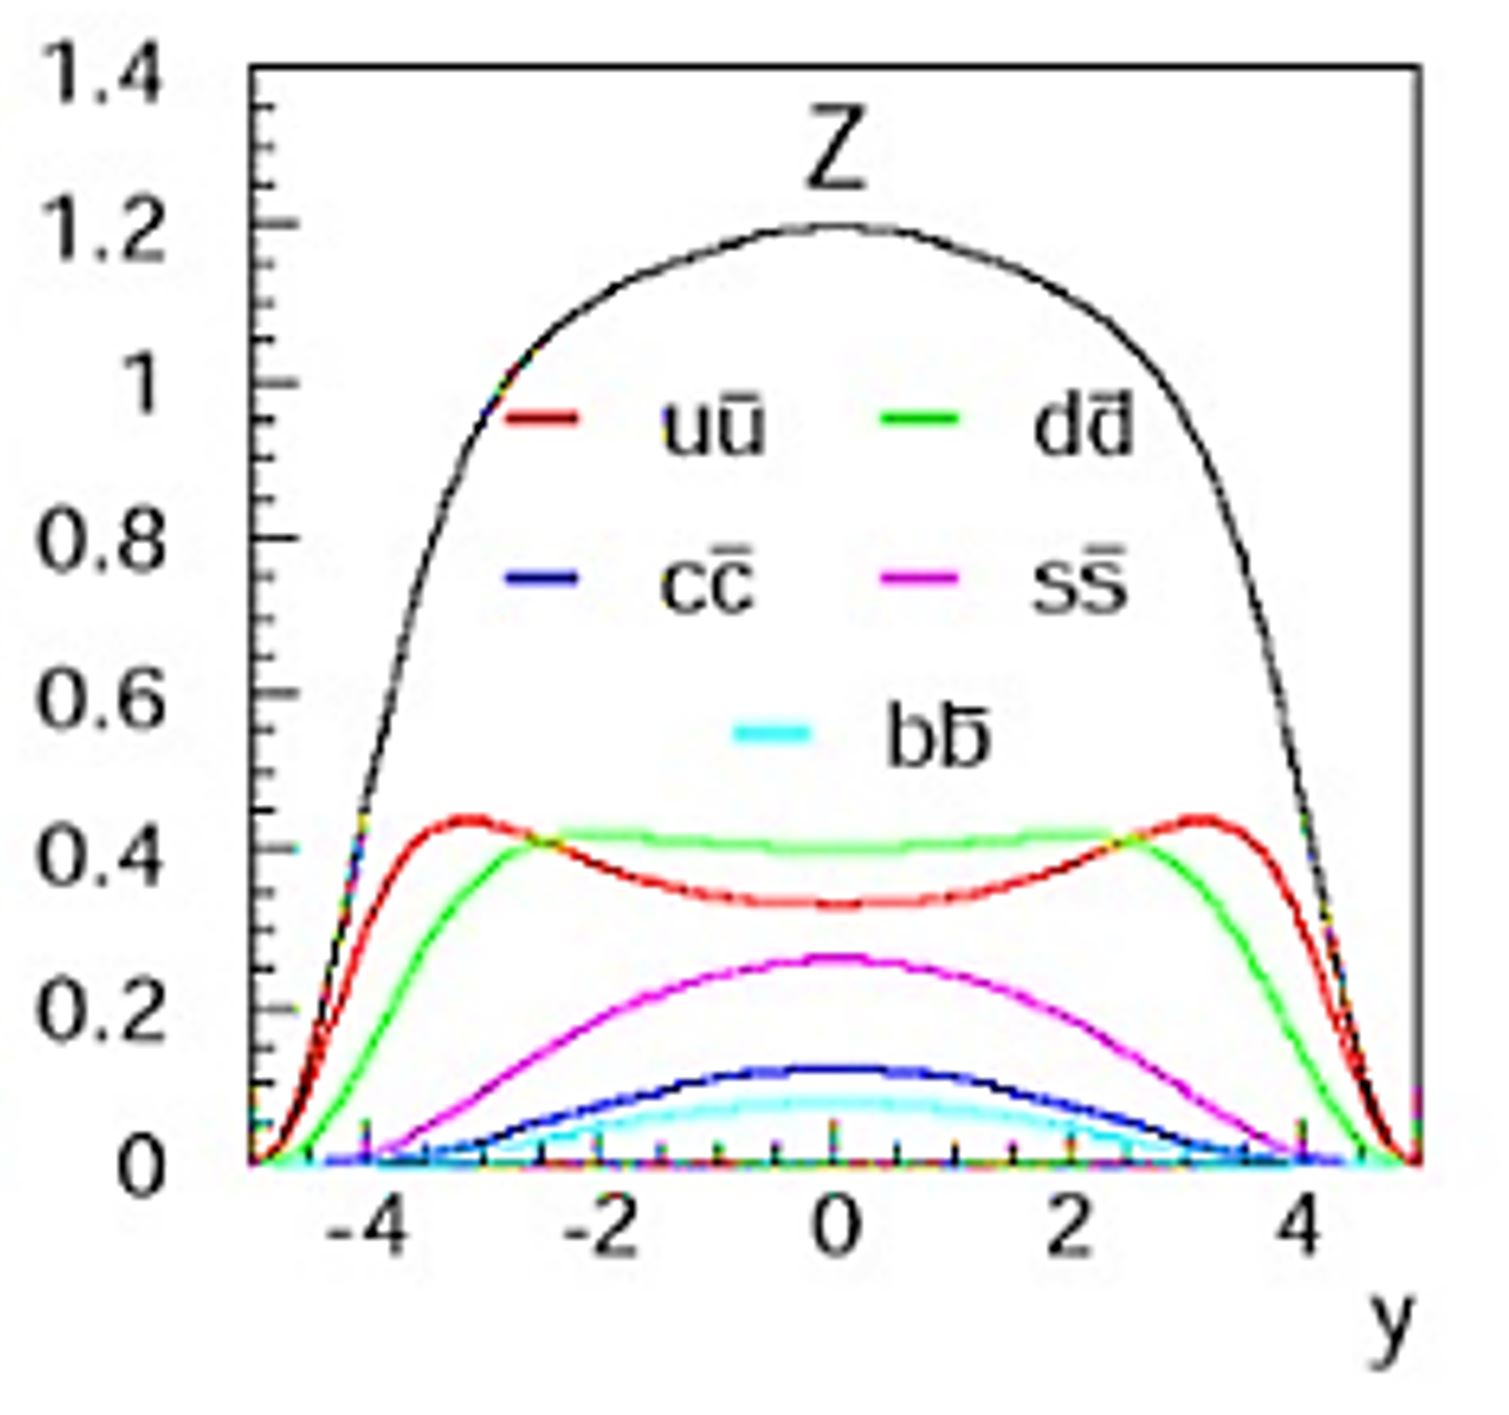
\includegraphics[width=0.32\textwidth]{plots/SM/rapidity_Z.JPG}
\caption{[Trying to make a new version from webplotdigitizer because these are ugly] Contribution of different quark flavors to the \Wp, \Wm, and \Z boson production over a range of boson rapidities. \Wp (\Wm) boson production is predominantly $u\bar{d}$ ($\bar{u}d$), while \Z boson production includes larger contributions from heavier flavors.}
\label{fig:wz_rapidity}
\end{figure}